\documentclass[aspectratio=1610]{beamer}
%[aspectratio=169]
% ------------------------------------------------------------------------
% PRAESENTATIONSAUSWAHL
\usecolortheme[RGB={3,138,94}]{structure} 
\mode<presentation> {
	%\usetheme{CambridgeUS} 
	\usetheme{Warsaw} 
	% oder Antibes, Bergen, Berkeley, ....
	
	%\setbeamercovered{transparent}
	
}
\useoutertheme{infolines}
\setbeamertemplate{headline}{}

\beamertemplatenavigationsymbolsempty
\definecolor{unigruen}{RGB}{3,138,94} 

\usefonttheme{professionalfonts}  % Aenderung der Schriftart
% (bei mathematischen Ausdruecken)
% ------------------------------------------------------------------------


% ------------------------------------------------------------------------
% EINGEBUNDENE PAKETE
\usepackage{xcolor}
\usepackage{varwidth}
\usepackage[utf8]{inputenc}
\usepackage{times,relsize,xspace}
\usepackage[T1]{fontenc}
\usepackage{mathtools}
\usepackage{dirtytalk}
\usepackage{minted,hyperref}

\hypersetup{
	colorlinks   = true,
}

\usepackage[style=authortitle,]{biblatex} %Imports biblatex package
\addbibresource{bibliography.bib} %Import the bibliography file
% Oder was auch immer. Zu beachten ist, das Font und Encoding passen
% muessen. Falls T1 nicht funktioniert, kann man versuchen, die Zeile
% mit fontenc zu loeschen.
% ------------------------------------------------------------------------

\newtheorem{thm}{Theorem}[theorem]

% ------------------------------------------------------------------------

\newcommand{\Rplus}{\protect\hspace{-.1em}\protect\raisebox{.35ex}{\smaller{\smaller\textbf{+}}}}
\newcommand{\Cpp}{\mbox{C\Rplus\Rplus}\xspace}

% Define the centeredblock environment to accept an optional argument for width
\newenvironment{centeredblock}[2][0.8\textwidth]
{ % This code will be executed at the beginning of the environment
	\begin{center}
		\begin{varwidth}{#1} % Use the argument for width
			\begin{block}{#2}
				\centering
			}
			{ % This code will be executed at the end of the environment
			\end{block}
		\end{varwidth}
	\end{center}
}


\title{Sequential and Parallel Debugging}
\subtitle{}
\author{Jonathan Schmalfuß}
\institute[UBT]{Chair of Scientific Computing \\ University of Bayreuth}
\date{\today}
%\tiny A talk adapt from \href{hackingcpp.com}{hackingcpp}

\begin{document}
	
	% TITELSEITE
	{
		\setbeamertemplate{headline}{} % Bei der Titelseite keine Kopf- und
		\setbeamertemplate{footline}{} % Fusszeile
		\begin{frame}
			\pagestyle{empty}
			\titlepage
			\pagestyle{empty}
		\end{frame}
	}
	
	\logo{} % remove logo from all following pages
	% Titelseite bei der Nummerierung ignorieren
	\addtocounter{framenumber}{-1}
	\setminted{fontsize=\footnotesize}
	
	\begin{frame}[fragile]{Sequential debugging}
		\begin{centeredblock}{}
			\say{Debugging is twice as hard as writing the code in the first place. Therefore, if you write the code as cleverly as possible, you are, by definition, not smart enough to debug it.} - Brian Kernighan, professor at Princeton University.
		\end{centeredblock}
	\end{frame}
	
	\begin{frame}[fragile]{Helpful compilation flags: g++ compiler}
		\begin{centeredblock}[0.85 \textwidth]{Warning flags}
			\begin{itemize}
				\item \texttt{-Wall}: Enables many warning flags
				\item \texttt{-Werror}: Converts any warning into an error
				\item \texttt{-Wextra}/\texttt{-W}: Additional warnings not in \texttt{-Wall}
				\item \texttt{-pedantic}/\texttt{-Wpedantic}: ISO standard compliance warnings
				\item Specific warnings:
				\begin{itemize}
					\item \texttt{-Wconversion}, \texttt{-Wcast-align}, \texttt{-Wunused}, \texttt{-Wshadow}, \texttt{-Wold-style-cast}
					\item \texttt{-Wpointer-arith}, \texttt{-Wcast-qual}, \texttt{-Wmissing-prototypes}, \texttt{-Wno-missing-braces}
				\end{itemize}
				
				\item the more the better, but only if you resolve them -  \href{https://github.com/cpp-best-practices/cppbestpractices/blob/master/02-Use_the_Tools_Available.md#gcc--clang}{Recommended Flags}
				\item use at least: \texttt{-Wall -Wextra -Wshadow -Wnon-virtual-dtor -pedantic}
			\end{itemize}
		\end{centeredblock}
		
		{\def\thefootnote{}\footnotetext{\href{https://caiorss.github.io/C-Cpp-Notes/compiler-flags-options.html}{CPP/C++ Compiler Flags and Options}}}
	\end{frame}
 
	\begin{frame}[fragile]{Trivial example: \texttt{-Wall}}
		\begin{centeredblock}[0.85 \textwidth]{}
			\inputminted{cpp}{../../02_programs/01_simplistic_introduction/wall_example.cpp}
		\end{centeredblock}
		
		\begin{centeredblock}[0.85 \textwidth]{}
			\begin{minted}{shell-session}
$ g++ wall_example.cpp
$ g++ -Wall -Werror wall_example.cpp
wall_example.cpp: In function 'int main()':
wall_example.cpp:5:55: error: 'x' is used uninitialized
5 |     std::cout << "Uninitialized value of x: " << x << "\n";
  |                                                       ^~~~
cc1plus: all warnings being treated as errors
			\end{minted}
		\end{centeredblock}
	
	\end{frame}

	
	\begin{frame}[fragile]{Debugger Frontends}
		\begin{centeredblock}[0.85 \textwidth]{}
			\begin{itemize}
				\item lightweight terminal based \href{https://cgdb.github.io/}{cgdb}
				\item old school \href{https://www.gnu.org/software/ddd/}{DDD}
				\item python based - browser-based \href{https://www.gdbgui.com/}{gdbgui}
				\item modern interpretation \href{https://github.com/epasveer/seer}{seer}
			\end{itemize}
			\begin{itemize}
				\item common wisdom: learn one, then others are easier to learn
			\end{itemize}
			\begin{columns}
				\column{0.5\textwidth}
				\centering
				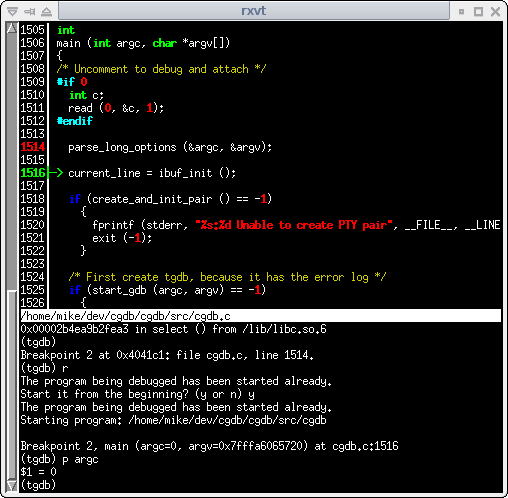
\includegraphics[width=0.7\linewidth]{images/cgdb.png}
				
				\column{0.5\textwidth}
				\centering
				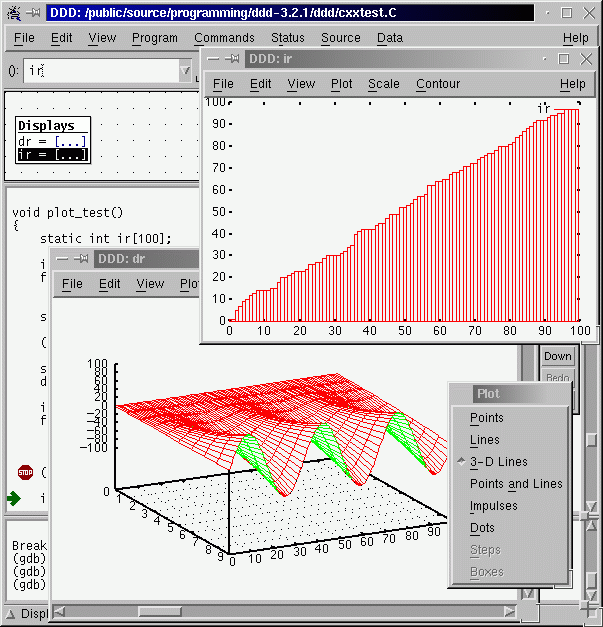
\includegraphics[width=0.7\linewidth]{images/DDD.png}
			\end{columns}
		\end{centeredblock}
	\end{frame}
	
	\begin{frame}[fragile]{All hail the king: GNU command line debugger: gdb}
		\begin{columns}
			\begin{column}{0.3\textwidth}
				\begin{block}{}
					\inputminted[firstline=1,lastline=12]{cpp}{../../02_programs/01_simplistic_introduction/gdb_factorial_example.cpp}
				\end{block}
			\end{column}
			\hfill
			\begin{column}{0.65\textwidth}
				\begin{block}{}
					\inputminted[firstline=14,lastline=23]{cpp}{../../02_programs/01_simplistic_introduction/gdb_factorial_example.cpp}
				\end{block}
			\end{column}
		\end{columns}
		\begin{centeredblock}[0.75 \textwidth]{}
			Live session inspired by \href{https://hackingcpp.com/cpp/tools/gdb_intro.html}{hackingcpp: Debugging With gdb}
		\end{centeredblock}
	\end{frame}
	
	\begin{frame}[fragile]{GNU command line debugger: gdb}
		\begin{block}{}
			\begin{table}[h!]
				\small
				\centering
				\begin{tabular}{|l|l|p{7.5cm}|}
					\hline
					\textbf{key / command}      & \textbf{short form} & \textbf{meaning}                                  \\ \hline
					\texttt{<Enter>}            &                     & repeat previous command                           \\ \hline
					\texttt{<Tab>}              &                     & complete command or function name                \\ \hline
					\texttt{run [<arg>...]}     & \texttt{r [<arg>...]} & run program (with command line argument(s))       \\ \hline
					\texttt{break <loc>}        & \texttt{b <loc>}    & set breakpoint at beginning of function or at a specific line \\ \hline
					\texttt{step}               & \texttt{s}          & next instruction, step into function             \\ \hline
					\texttt{next}               & \texttt{n}          & next instruction, step over function             \\ \hline
					\texttt{jump <loc>}         & \texttt{j <loc>}    & jump to location (useful for exiting long/endless loops) \\ \hline
					\texttt{continue}           & \texttt{c}          & continue until next breakpoint or end of program \\ \hline
					\texttt{until <loc>}        & \texttt{u <loc>}    & continue until location (function /line)         \\ \hline
					\texttt{finish}             & \texttt{fin}        & finish (step out of) current function            \\ \hline
					\texttt{print <expression>} & \texttt{p}          & print value of expression, e.g., variable        \\ \hline
					\texttt{info breakpoints}   & \texttt{i b}        & list all breakpoints                             \\ \hline
					\texttt{info locals}        & \texttt{i locals}   & list local variables and their values            \\ \hline
					\texttt{backtrace}          & \texttt{bt}         & show call stack                                  \\ \hline
				\end{tabular}
				\caption{Useful gdb Commands}
				\label{table:gdb_commands}
				\vspace{-0.5cm}
			\end{table}
		\end{block}
	\end{frame}
	
	\begin{frame}[fragile]{Valgrind's tool suite}
		\begin{centeredblock}[0.85 \textwidth]{}
			\begin{itemize}
				\item Memcheck: detects memory-management problems: \newline 
					\texttt{valgrind --leak-check=full --show-leak-kinds=all --track-origins=yes --verbose <myexecutable>}
					\item example usage
\begin{minted}{shell-session}
$ g++ -g Wall -Werror out_of_bounds.cpp -o out_of_bounds.out
$ valgrind ./out_of_bounds.out
==182905== Memcheck, a memory error detector
==182905== Copyright (C) 2002-2022, and GNU GPL'd, by Seward et al.
==182905== Using Valgrind-3.21.0 and LibVEX;
==182905== Command: ./a.out
==182905== 
==182905== Invalid read of size 8
...
\end{minted}
			\end{itemize}
		\end{centeredblock}
	\end{frame}
	
	\begin{frame}[fragile]{Sanitizers}
		\begin{centeredblock}{Sanitizers}
			\begin{itemize}
				\item AddressSanitizer - memory error detector: \texttt{-fsanitize=address} 
				\item UndefinedBehaviorSanitizer - undefined behavior detector: \texttt{-fsanitize=undefined}
				\item ThreadSanitizer - data race detector: \texttt{-fsanitize=thread}
			\end{itemize}
		\end{centeredblock}
	
		{\def\thefootnote{}\footnotetext{\href{https://gcc.gnu.org/onlinedocs/gcc/Instrumentation-Options.html#index-fsanitize_003daddress}{GCC compiler flags for fsanitize}}}
	\end{frame}
	
	\begin{frame}[fragile]{Example: Sanitizers}
		\begin{centeredblock}[0.95 \textwidth]{}
			\begin{minted}{shell-session}
$ g++ -g -fsanitize=address segfault.cpp -o a_segfault.out
$ ./a_segfault.out
AddressSanitizer:DEADLYSIGNAL
=================================================================
==188435==ERROR: AddressSanitizer: SEGV on unknown address 0x000000000000
...

==188435==ABORTING
			\end{minted}
		\end{centeredblock}
	\end{frame}
	
	\begin{frame}[fragile]{Honorable Mentions: Static analyzers / Linters}
		
		\begin{centeredblock}{Honorable Mentions: Static analyzers / Linters}
			\begin{itemize}
				\item cppcheck
				\item Clang-Tidy
			\end{itemize}
		\end{centeredblock}
	\end{frame}
	
	\begin{frame}[fragile]{Time travel debugging}
		\begin{centeredblock}{}
			Idea: run gdb; stop at the point where problem occurs; walk backwards figure out what happend
			
			$\Rightarrow$ theoretically supported by gdb via commands such as \texttt{reverse-next}
			\begin{itemize}
				\item Problem: avx instruction $\Rightarrow$ unusable most of the time
				\item Solution: \texttt{rr}\footnote{\href{rr}{https://rr-project.org/}}: record a failure once, then debug the recording, deterministically, as many times as you want
			\end{itemize}
		\end{centeredblock}
	\end{frame}

\begin{frame}[fragile]{Now what?}
	\begin{block}{Use the tools / test them on simple and more complex examples}
		In the corresponding \href{https://github.com/joscao/cpp-debugging}{github project} work through the folder \texttt{02\_sequential\_programs} content. The available tools on the PC-Pool workstations are gdb / sanitizer / valgrind.
	
		\vspace{1cm}
	
		Possible tasks:
		\begin{itemize}
			\item How many bugs can be found using only the warning flags? Is there a special type that is difficult to be found using warning flags?
			\item Learn to read the sanitizer / valgrind output. Attempt the trivial examples first, then try the more difficult ones.
			\item Hints / Solutions are available for the more complicated one, use them!
			\item Last but not least: Ask Questions, not only to me but also to each other about your understanding.
		\end{itemize}
	\end{block}
\end{frame}
\end{document}